Please see Appendix, Table \ref{tb:patient-classification} for PR values and classification of each patient.

\begin{figure}[h]
    \centering
    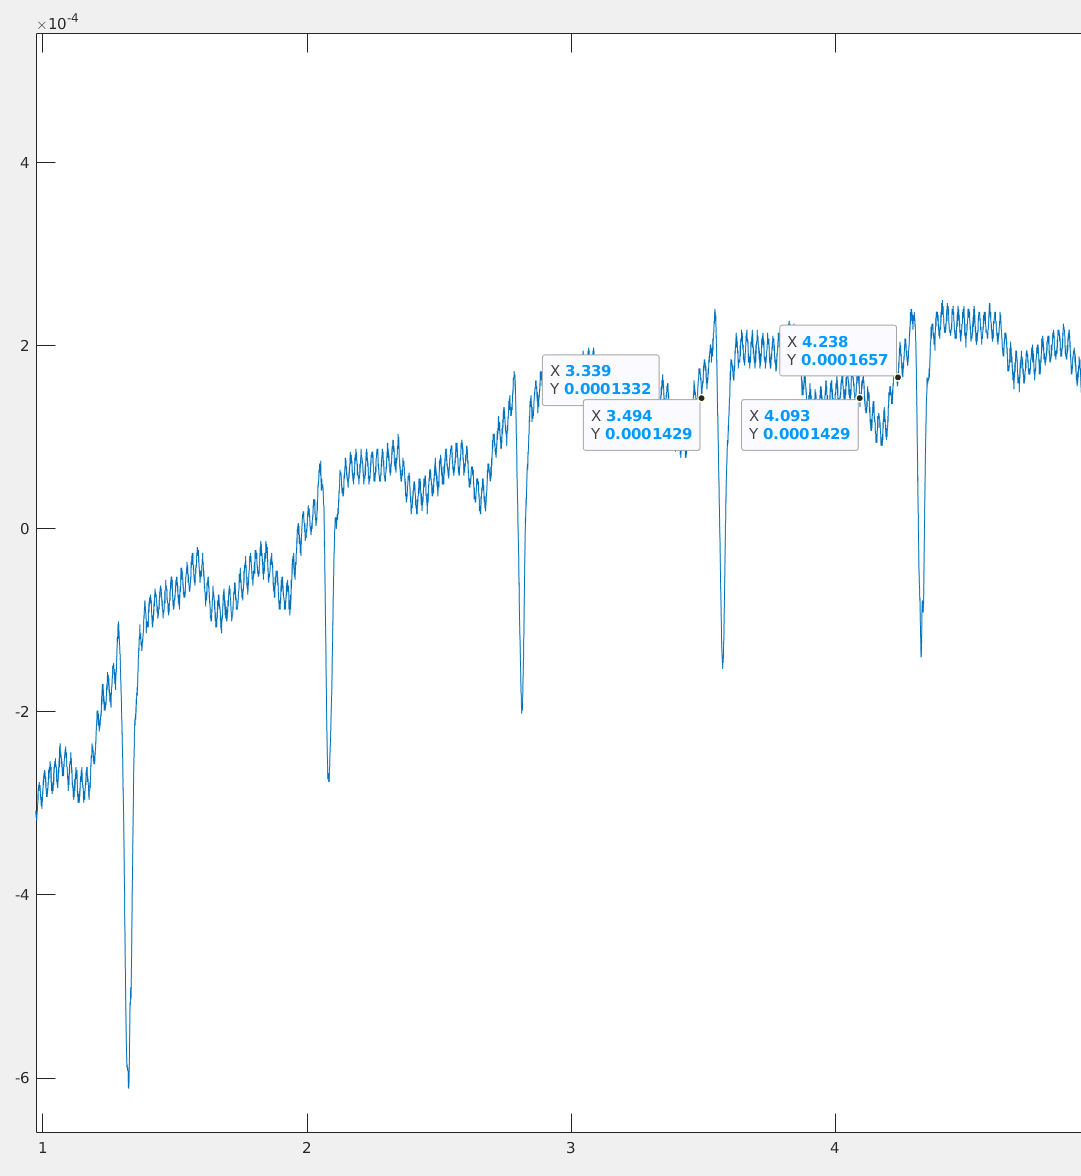
\includegraphics[width=0.8\textwidth]{Defining_PR.png}
    \caption{Using Matlab to estimate PR length. Notice the amount of noise, increasing uncertainty. Code in Appendix, Listing \ref{ls:genData}.}
    \label{}
\end{figure}

\begin{table}[h]
    \centering
\begin{tabular} {ccc}
& \multicolumn{2}{c}{\textbf{Definitive Diagnosis}} \\
\toprule
\textbf{Diagnostic test} &   Abnormal & Normal \\
\midrule
Abnormal        &      2    & 5 \\
Normal          &      4    & 19 \\
\bottomrule
\end{tabular}
\caption{Comparison between gold standard and analysis using analogue filter circuit.}
\end{table}
From which we may calculate:
\begin{equation}
\begin{split}
    \text{Sensitivity} &= \frac{2}{6} = 33.33\% \\
    \text{Specificity} &= \frac{19}{24} = 79.16\%
\end{split}
\end{equation}

These results imply that 30\% ($\frac{9}{30}$) of all patients would be given an incorrect diagnosis.
Ethically a clinician could not present a diagnosis made solely with this circuit -- especially given that it only caught first-degree heart block (FDHB) in $\frac{1}{3}$ of cases.
Given the expectation that this filter arrangement was poor, this inaccuracy is unsurprising, but at the same time it is encouraging that true negatives were caught 79\% of the time -- perhaps making this valuable purely in supporting a negative diagnosis.
Analogue circuits are, nevertheless, valuable for their simplicity and accomplishing the reduction of interference, which this circuit has (to some extent) successfully done.

Alternatively, one supplements the use of analogue circuits with digital filtering.
There are several algorithms that attempt to perform the task -- some more successful than others \citep{GarciaManuel2018Anwf}.
Even filters with the ability to produce adaptive filtration, varying with the dynamic range of an ECG, have relatively low complexity -- though they require hard-to-obtain external references \citep{GarciaManuel2018Anwf}.
Indeed, this is a field in continuous development, and ultimately both analogue and digital filtration has to be used in conjunction.